\documentclass{beamer}
\usepackage[utf8]{inputenc}
\usepackage{hyperref}
%\usepackage{minted}\\
\usepackage{csvsimple}

\graphicspath{{img/}}
\bibliographystyle{alpha}

\title[Summary]{Systematic Mapping Study on Megamodels}
\author{Matthias Barde \& Marco Brack, University of Koblenz-Landau}
\institute{SLE course SS 2016 (\url{http://www.softlang.org/course:sle16})}
\date{2016-06-16}

\addtobeamertemplate{navigation symbols}{}{%
    \usebeamerfont{footline}%
    \usebeamercolor[fg]{footline}%
    \hspace{1em}%
    \insertframenumber/\inserttotalframenumber
}

\begin{document}

\begin{frame}
\titlepage
\end{frame}


\begin{frame}{Definition}
\begin{figure}
  \textit{``Megamodeling is the activity of specifying systems of models and mappings, their properties, and operations over them.''} \cite{diskin2013mapping}

  \pause
  \vspace{1cm}
  Or is it?
\end{figure}
\end{frame}


\begin{frame}{Systematic Mapping Study}
\begin{figure}
	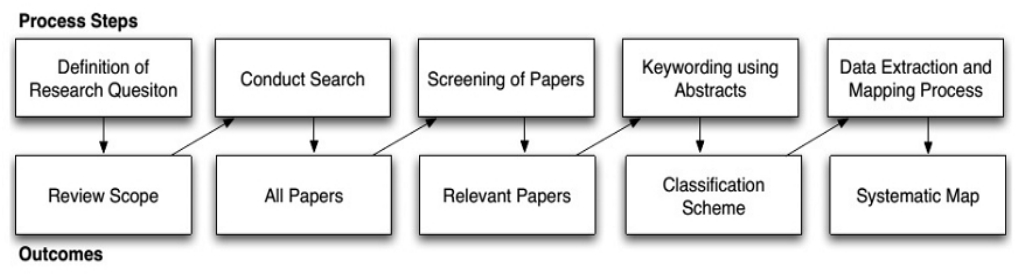
\includegraphics[width=1.0\textwidth]{sms_full}
	\caption{From \textit{Literature Studies in Software Engineering} \cite{litstud}}
\end{figure}
\end{frame}

\begin{frame}{Systematic Mapping Study}
\begin{figure}
	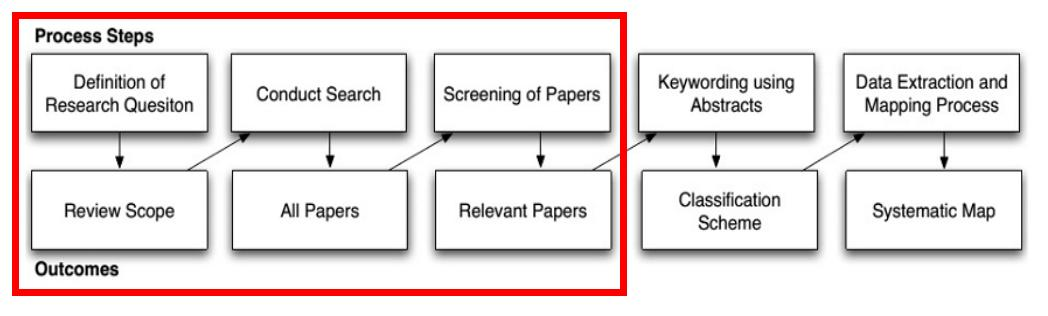
\includegraphics[width=1.0\textwidth]{sms_part_marked}
\end{figure}
\end{frame}

\begin{frame}{Research Questions}
\begin{enumerate}
	\item How do researchers define megamodeling?
	\item What kinds of model elements are used?
	\item Which practical purposes do the megamodels serve, if any?
	\item Which technology is used to implement the megamodels?
\end{enumerate}
\end{frame}

\begin{frame}{Research Question 1}
\begin{tabular}{|l|p{9cm}|}\hline
\textbf{RQ 1} & How do researchers define megamodeling?\\\hline
\textbf{Why?} & There does not exist a common definition of me\-ga\-mo\-dels to which everyone relates to. So it is interesting to get an overview over how different researchers define megamodels.\\\hline
\textbf{How?} & Check if papers provide whether an explicit or implicit definition of megamodels.\\\hline
\end{tabular}
\end{frame}

\begin{frame}{Example}
From introduction of \textit{Toward Mega Models for Maintaining Timing Properties of Automotive Systems} \cite{Neumann_models2010}:
\begin{center}
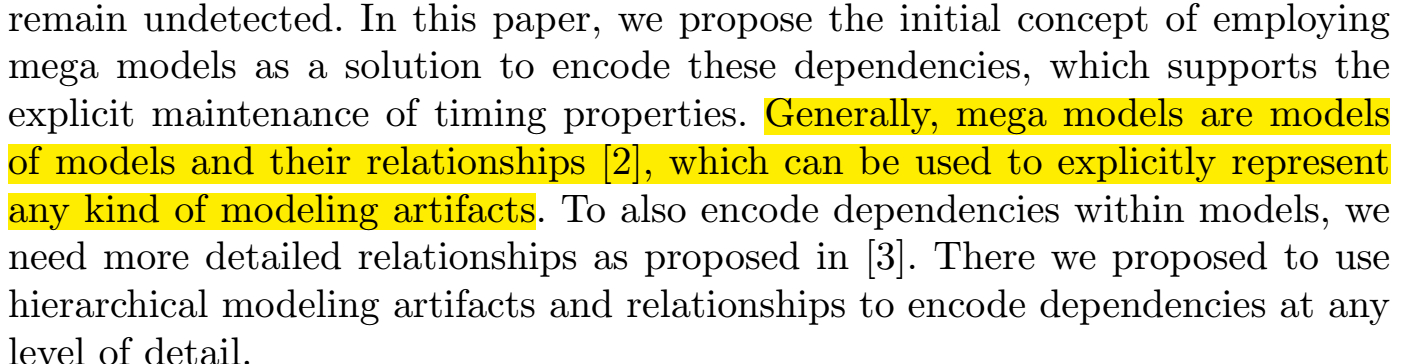
\includegraphics[width=1.0\textwidth]{ex_rq1}
\end{center}
\end{frame}

\begin{frame}{Research Question 2}
\begin{tabular}{|l|p{9cm}|}\hline
\textbf{RQ 2} & What kinds of model elements are used?\\\hline
\textbf{Why?} & Megamodels have a wide range of imaginable application scenarios. Getting an overview over which elements are used in megamodels leads to an overview over which scenarios are covered by megeamodels.\\\hline
\textbf{How?} & Check if papers describe explicit or implicit which elements are used in given megamodels. This could be concrete or abstract elements.\\\hline
\end{tabular}
\end{frame}

\begin{frame}{Example}
From introduction of \textit{A Megamodel for Process Tailoring and Evolution} \cite{tailoring}:
\begin{center}
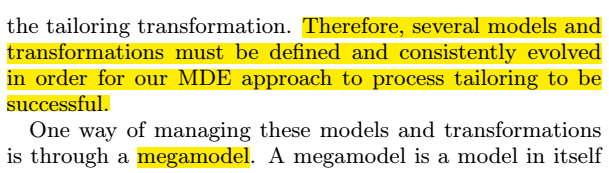
\includegraphics[width=1.0\textwidth]{ex_rq2}
\end{center}
\end{frame}

\begin{frame}{Research Question 3}
\begin{tabular}{|l|p{9cm}|}\hline
\textbf{RQ 3} & Which practical purposes do the megamodels serve, if any?\\\hline
\textbf{Why?} & It is interesting to get an overview for what megamodels can be used in practice.\\\hline
\textbf{How?} & Check if megamodels in the papers are 	instrumentalized to fulfill a concretely described practical purpose.\\\hline
\end{tabular}
\end{frame}

\begin{frame}{Example}
From abstract of \textit{A Megamodel for Process Tailoring and Evolution} \cite{tailoring}:
\begin{center}
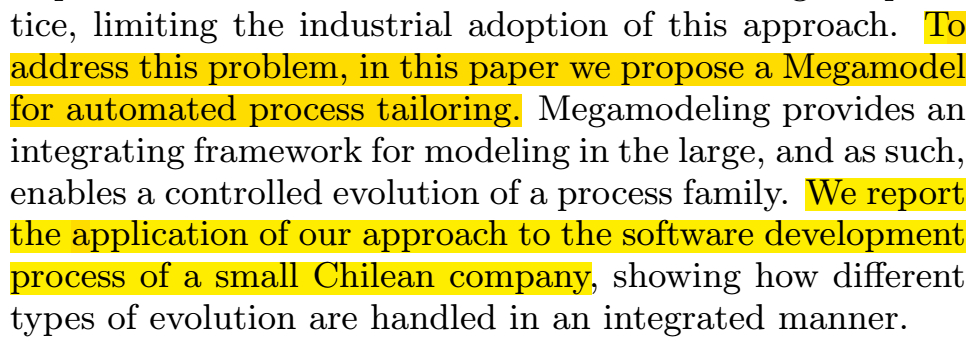
\includegraphics[width=1.0\textwidth]{ex_rq3}
\end{center}
\end{frame}

\begin{frame}{Research Question 4}
\begin{tabular}{|l|p{9cm}|}\hline
\textbf{RQ 4} & Which technology is used to implement the megamodels?\\\hline
\textbf{Why?} & Since megamodelling is a (relatively) new approach it is interesting to get an overview over existing technologies in this field.\\\hline
\textbf{How?} & Check if papers describe that mentioned megamodels were actually implemented. An implementation has to provide functionalities and some kind of reusability (i.e. a graphical representation of a megemodel is not an implementation).\\\hline
\end{tabular}
\end{frame}

\begin{frame}{Example}
From introduction of \textit{A Megamodel for Process Tailoring and Evolution} \cite{tailoring}:
\begin{center}
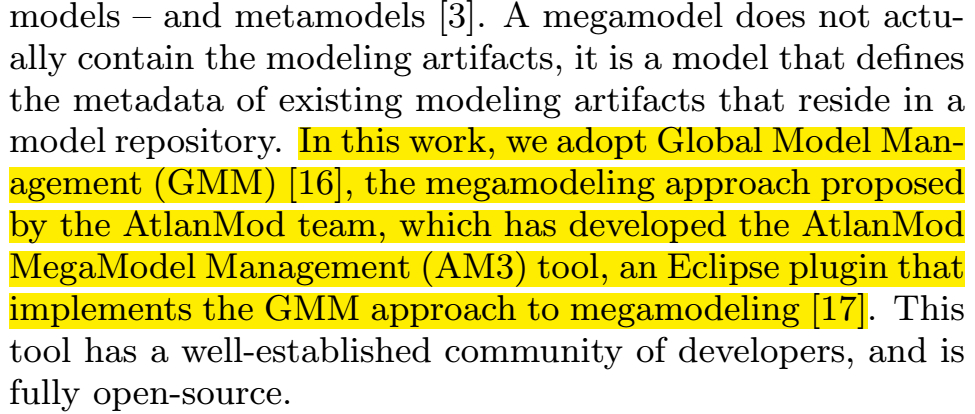
\includegraphics[width=1.0\textwidth]{ex_rq4}
\end{center}
\end{frame}

\begin{frame}{Review Scope \& Conduct Search}

\begin{block}{Scope}
\begin{itemize}
	\item Papers cited in \textit{An Abstract View on Megamodeling Approaches} by Ralf Lämmel and Vadim Zaytsev \footnote{\url{http://softlang.uni-koblenz.de/megamodeling-in-the-wild/}}
	\item Elsevier
	\item Springer
	\item IEEE
	\item ACM
	\item DLBP
	\item Google Scholar as search engine
\end{itemize}
\end{block}

\begin{block}{Search query}
\textit{megamodel}, \textit{megamodeling} or similar must be contained in title or abstract.
\end{block}

\end{frame}

% Show collected papers as list at least one time.
\begin{frame}{All papers I}
33 papers, from 1974 to 2015
\begin{figure}
	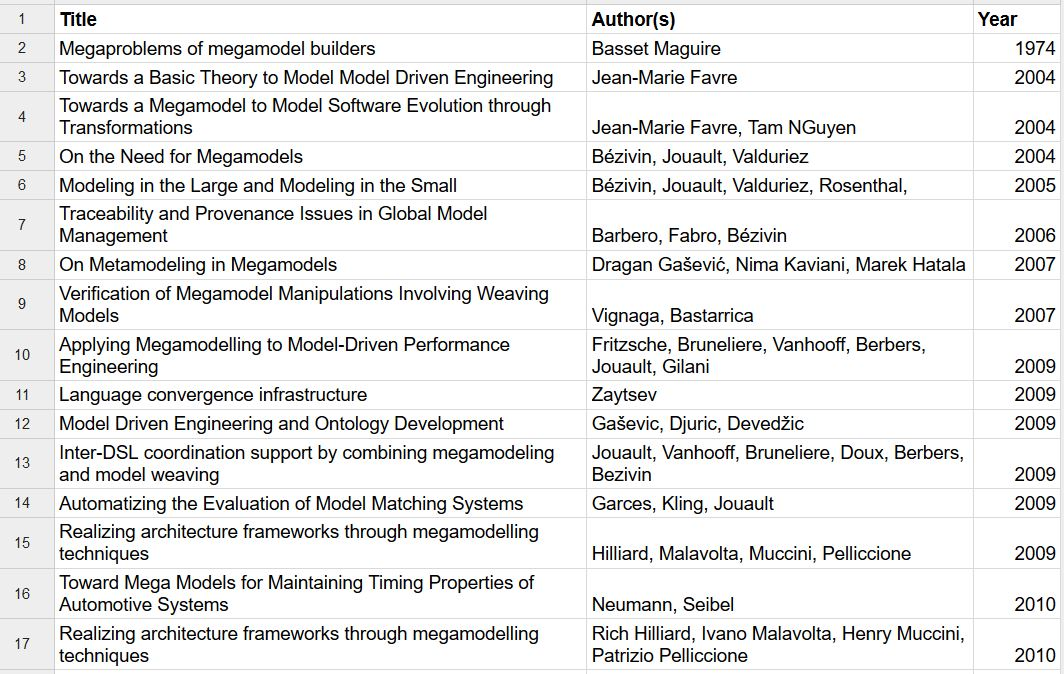
\includegraphics[width=1.0\textwidth]{all_papers_1}
\end{figure}
\end{frame}

\begin{frame}{All papers II}
\begin{figure}
	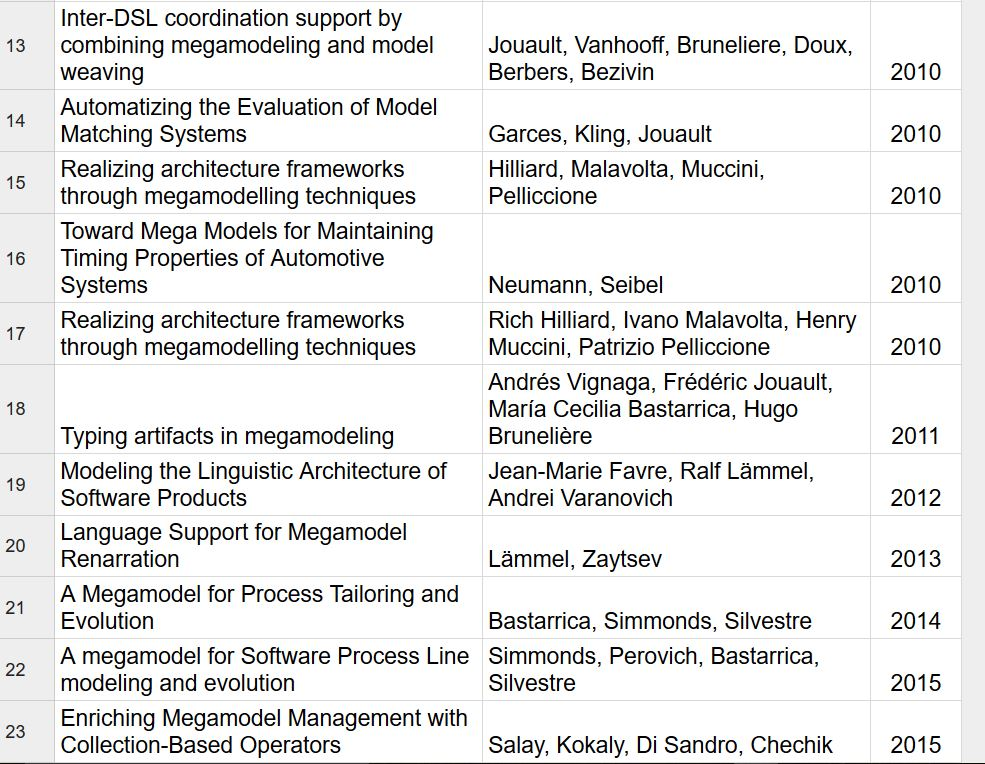
\includegraphics[width=1.0\textwidth]{all_papers_2}
\end{figure}
\end{frame}

\begin{frame}{Screening}
\begin{block}{Checking content of all papers:}
\begin{itemize}
	\item Abstract
	\item Introduction
	\item Conclusion
\end{itemize}
\end{block}
\vspace{1cm}
\large{$\rightarrow$ Can they contribute to our Research} Questions?\\
\large{$\rightarrow$ Short relevance analysis of each paper}
\end{frame}

\begin{frame}{Relevant papers}
\begin{itemize}
	\item Removed papers which do not contribute to any Research Question $\rightarrow$ \textit{Exclusion criterium}
	\item Number of papers reduced to 31
	\begin{itemize}
		\item 19 contribute to each Research Question
		\item 16 contribute to 3 or more Research Questions
	\end{itemize}
\end{itemize}

\end{frame}

\begin{frame}{Future steps}
\begin{figure}
	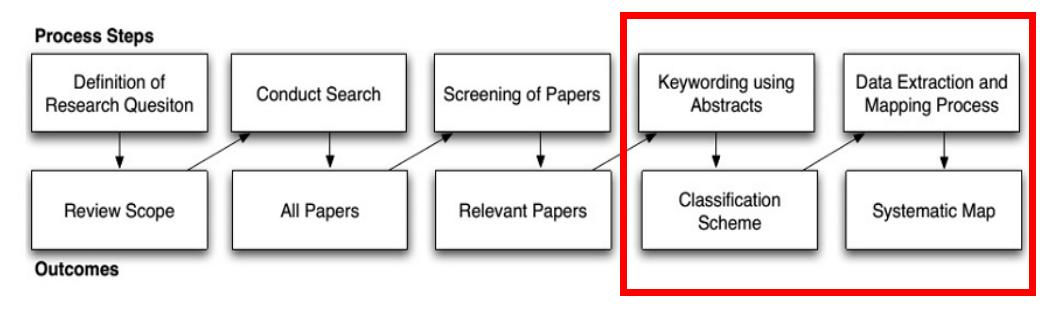
\includegraphics[width=1.0\textwidth]{sms_part_marked_2}
\end{figure}
\end{frame}

\begin{frame}
  \bibliography{slides}
\end{frame}

\begin{frame}
\begin{center}
	\huge{Thank You All For Listening}
\end{center}
\end{frame}

\end{document}
